\documentclass[aspectratio=169]{beamer}
\usepackage[utf8]{inputenc}
\usepackage{bookman}
\usetheme{Dresden}
\usepackage{graphicx}
\usepackage{hyperref}

\title[02-CAD]{Introduction to Computer Aided Design\\(3D Modeling)}
\author{Prototyping Skills (BME290L)}
\institute[Palmeri]{Mark L. Palmeri, M.D., Ph.D.}
\date{January 17, 2023}
\logo{
\includegraphics[width=0.1\textwidth]{BME-HorizontalLogo-Web-Blue.png}}

\begin{document}

\frame{\titlepage}

\frame{
    \frametitle{Outline}
    \tableofcontents
}

\frame{
    \frametitle{OnShape}

    \begin{center}
        
\includegraphics[width=0.33\textwidth]{logo-onshape-gray-green.png}
    \end{center}

    \begin{itemize}
        \item We will be using OnShape, a cloud-based CAD package with a similar
        workflow to SolidWorks.
        \item You have been automatically registered to join Duke's OnShape team
        (\url{https://duke.onshape.com}).
    \end{itemize}
}

\frame{

    \frametitle{Tutorials}

    \begin{itemize}
        \item OnShape
        \begin{itemize}
            \item \href{https://learn.onshape.com/courses/fundamentals-sketching}{Introduction to Sketching}
            \item \href{https://learn.onshape.com/courses/introduction-to-part-design}{Introduction to Part Design}
            \item \href{https://learn.onshape.com/courses/introduction-to-2d-drawings}{Introduction to 2D Drawings}
        \end{itemize}
        \item \href{https://www.hubs.com/knowledge-base/enclosure-design-3d-printing-step-step-guide/}{Enclosure Design for 3D Printing}
        \item \href{https://www.hubs.com/knowledge-base/how-assemble-3d-printed-parts-threaded-fasteners/}{How to assemble 3D printed parts with threaded fasteners}
        \item \href{https://www.hubs.com/knowledge-base/how-design-snap-fit-joints-3d-printing/}{How to design snap-fit joints for 3D printing}
    \end{itemize}
}

\section{General Workflow}

\frame{

    \frametitle{General Workflow}

    \begin{enumerate}
        \item Sketch 2D profiles (dimensioned).
        \item Use constraints to align sketch features to one another.
        \item Extend 2D profiles to 3D \underline{parts}.
        \begin{itemize}
            \item Extrude (new, add, subtract, intersection)
            \item Revolve
        \end{itemize}
        \item Utilize part symmetry and patterns to reduce manual effort.
        \item Define new sketch planes on part references that ``make sense''.
        \item Assemble multiple parts.
    \end{enumerate}
}

\frame{

    \frametitle{Practice Makes Perfect}

    \begin{itemize}
        \item There are many ways to create the same parts.  Some are more amenable to future modification than others; those aren't always the fastest to create from scratch.  
    
        \item Experience is highly valuable!
    \end{itemize}
}

\section{Modifying Edges}
\subsection{Common Types}

\frame{

    \frametitle{Modifying Edges}

    \begin{itemize}
        \item \underline{Fillet}: rounded corner / edge
        \item \underline{Chamfer}: sloped / angled corner / edge
    \end{itemize}

    \centerline{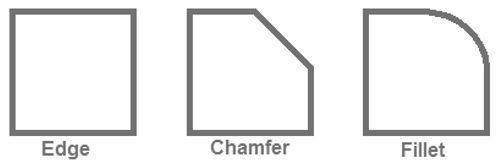
\includegraphics[width=0.5\textwidth]{edge_chamfer_fillet.jpg}}
    \centerline{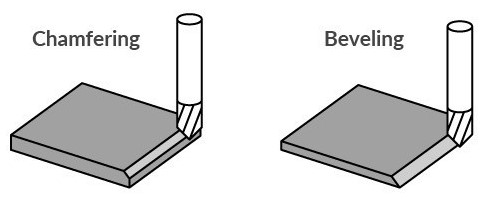
\includegraphics[width=0.5\textwidth]{chamfering_beveling.jpg}}

}

\subsection{Why?}
\frame{
    \frametitle{Why modify edges?}

    \begin{itemize}
        \item Reduce stress concentrations (fillet $>$ chamfer).
        \item Reduce sharp edges.
        \item Ease assembly (potentialy at cost to manufacturing).
    \end{itemize}

    \centerline{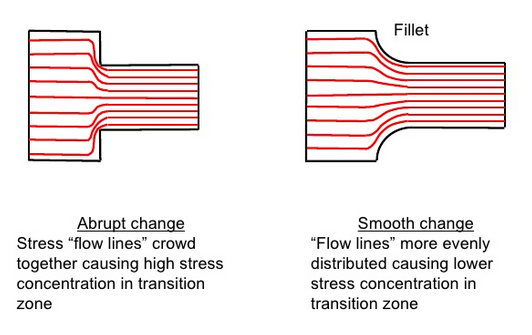
\includegraphics[width=0.5\textwidth]{stress_concentration.png}}
}

% TODO: Add picture of Hole tool in OnShape
\section{Holes}
\frame{

    \frametitle{Types of Holes}
    \centerline{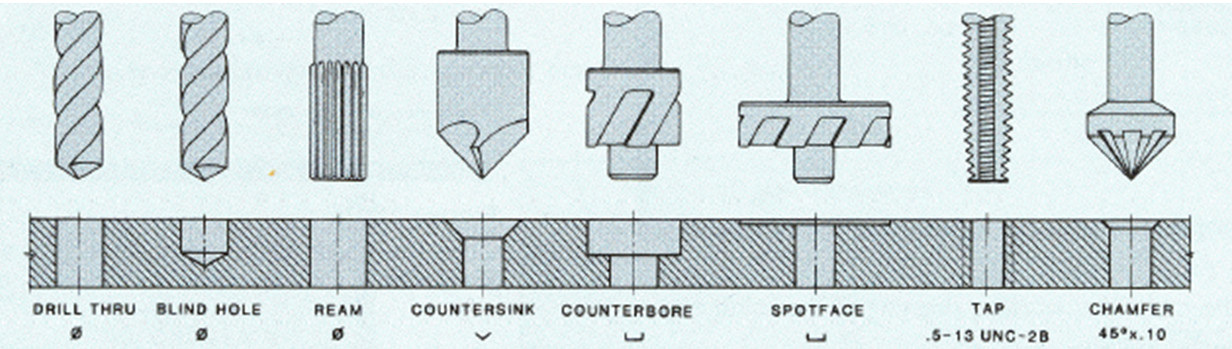
\includegraphics[width=1.0\textwidth]{holes.jpg}}

CAD software has a specific
\href{https://cad.onshape.com/help/Content/hole.htm}{Hole} tool that can be very
handy.  Specify diameters and threading based on ANSI and ISO standards (e.g.,
ANSI \#10-32 bolt or ISO M5-0.8).  Additionally, a table of holes can be
generated on mechanical drawings.

}

\subsection{Screws}
\frame{

    \frametitle{Types of Screws}

    \centerline{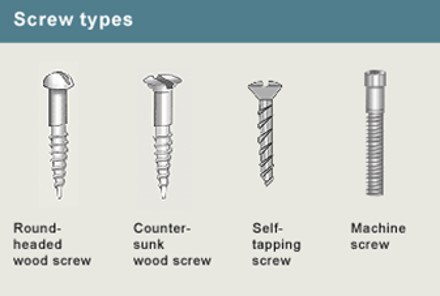
\includegraphics[width=0.5\textwidth]{screws.jpg}}

}

\section{Mechanical Drawings}

\frame{
    \frametitle{Mechanical Drawings}

    \begin{columns}
        \begin{column}{0.5\textwidth}
            \begin{itemize}
                \item Multiview / orthographic projection
                \item ISO 8015 (``Geometrical product specifications (GPS) — Fundamentals — Concepts, principles and rules'')
                \item Dimension callouts / values should not overlap any part lines!
            \end{itemize}
        \end{column}
        \begin{column}{0.5\textwidth}
            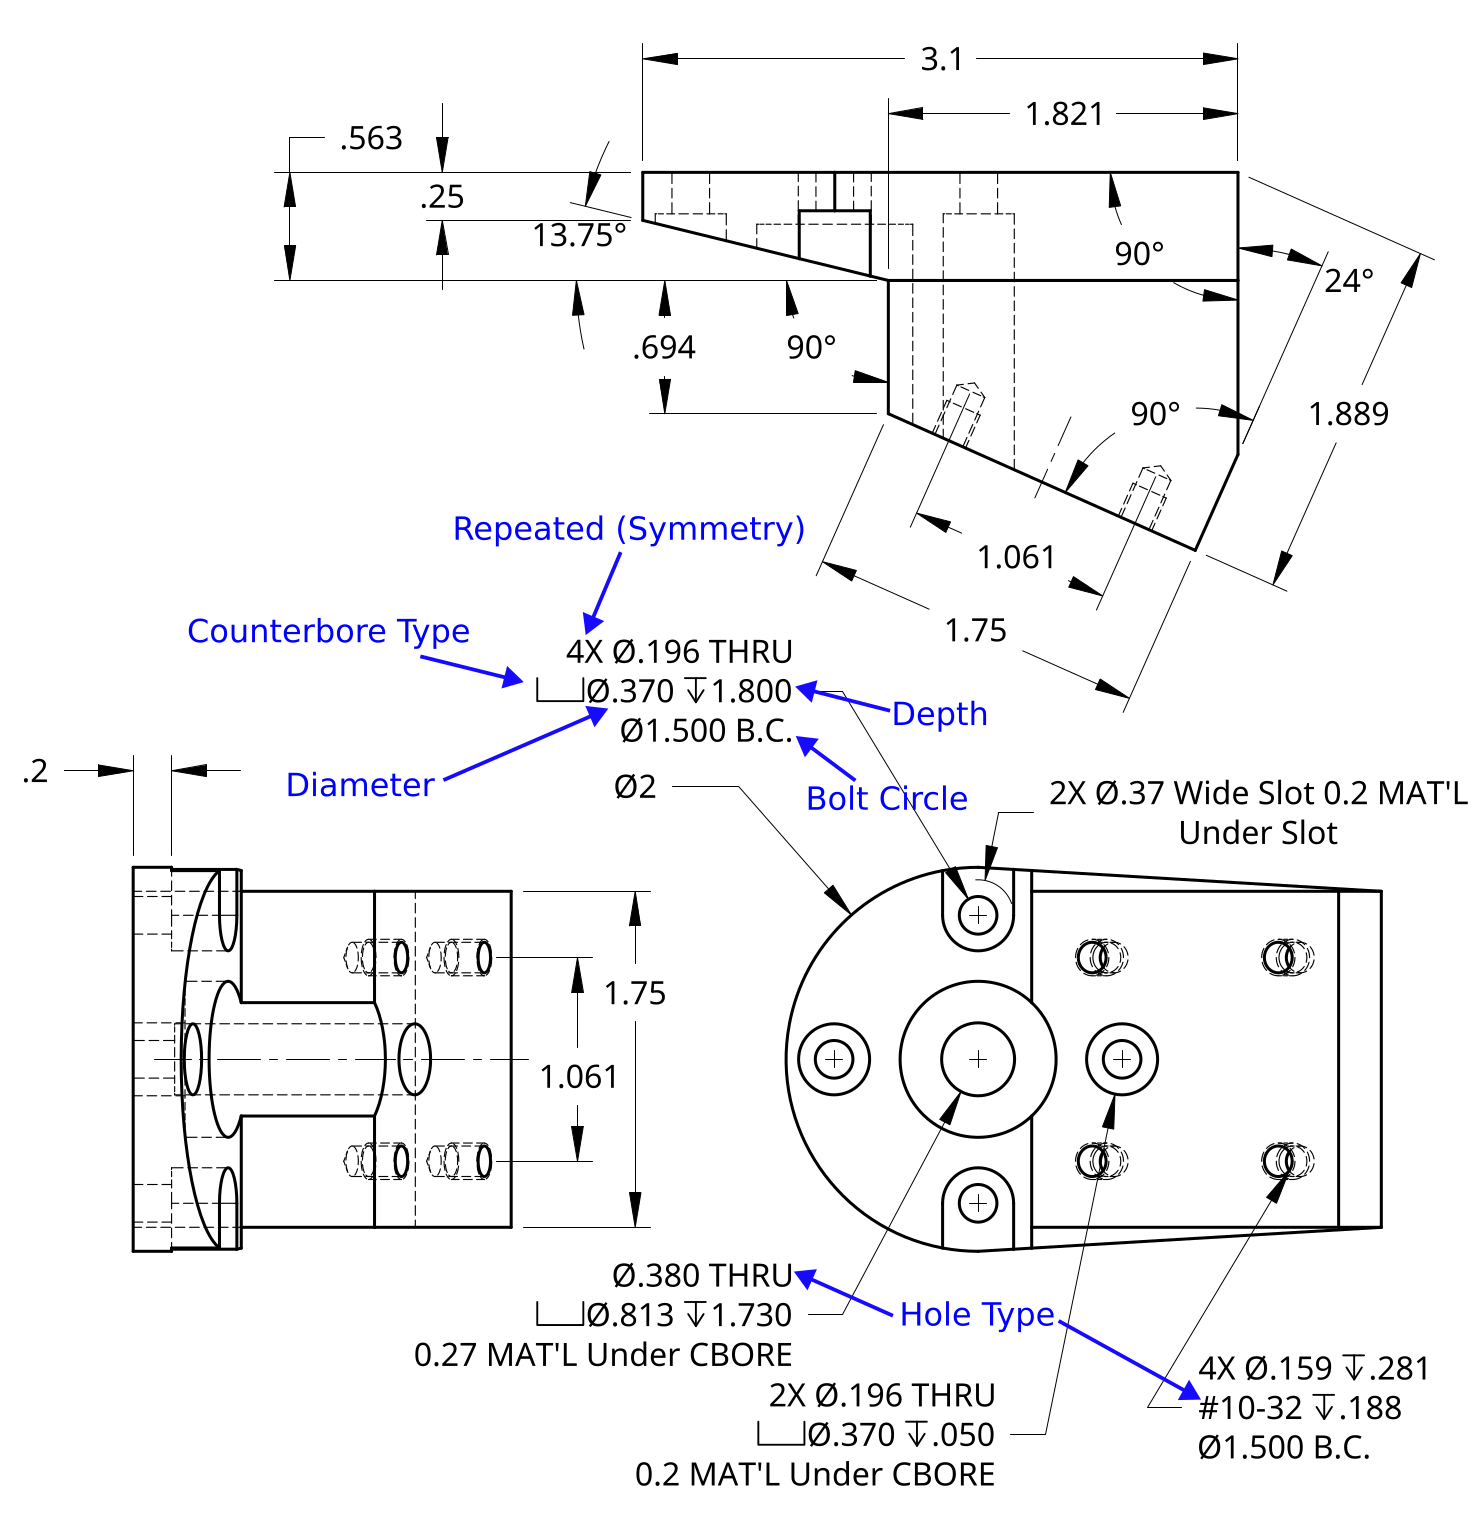
\includegraphics[width=0.85\textwidth]{mechanical_drawing_annotated.png}
        \end{column}
    \end{columns}

}

\section{Mechanical Design Considerations}
\frame{

    \frametitle{Mechanical Design Considerations}
    \begin{itemize}
        \item Purpose
        \begin{itemize}
            \item Protection (water, debris?)
            \item Holding components in relation to each other
            \item Mounting
        \end{itemize}
        \item Loading
        \begin{itemize}
            \item Shipping
            \item Gravity / Momentum
            \item Falls (especially corners)
            \item Buttons
        \end{itemize}
        \item Interfaces
        \begin{itemize}
            \item Cables
            \item Displays
            \item Buttons
        \end{itemize}
        \item Minimize all else!
    \end{itemize}
}

\section{Demo}

\begin{frame}
    \frametitle{Flange}

    \begin{columns}
        \begin{column}{0.6\textwidth}
            What is a \textbf{flange}?
            \begin{itemize}
                \item Internal/external ridge/lip/rim
                \item $\Uparrow$ \textbf{strength} / distribute \textbf{contact force} between mating pieces
                \item Commonly uses a \textbf{bolt circle} (BC)
            \end{itemize}
        \end{column}
    \begin{column}{0.4\textwidth}
        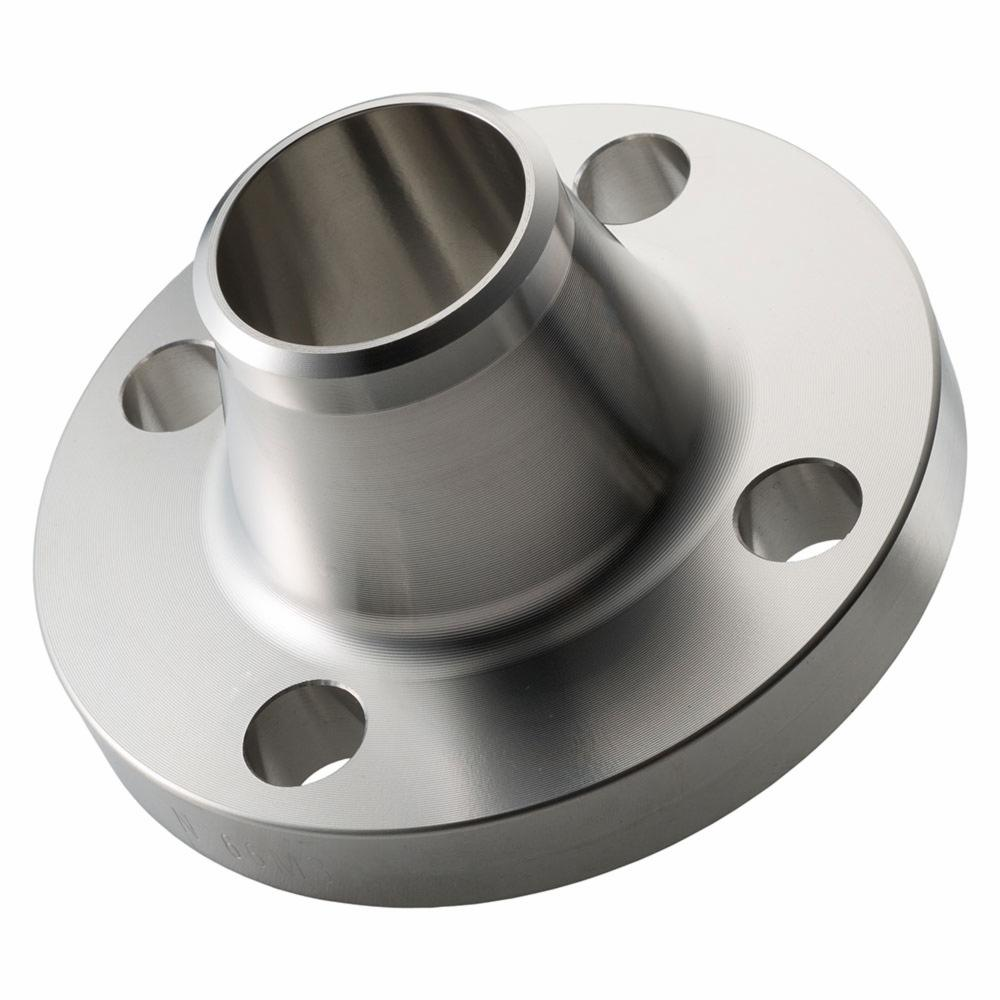
\includegraphics[width=1.0\textwidth]{example_flange.jpg}
    \end{column}
    \end{columns}
    
\end{frame}

\begin{frame}
    \begin{itemize}
        \item \href{https://duke.onshape.com/documents/b3956eb8825462298489e96a/w/edf0f27c18c0a0fca15f1917/e/98b7c112763862d14bb59aef?renderMode=0&uiState=63c5907e33f5773100e9598d}{Demo}
        \item Tips:
        \begin{itemize}
            \item Rename steps to build the part
            \item Use variables for dimensions that may change
            \item Use patterns when possible
            \item Note version history / tag specific revisions
            \item Look at different views, including ``sections''
            \item Create mechanical drawing
        \end{itemize}
    \end{itemize}
\end{frame}

\begin{frame}
    \begin{columns}
        \begin{column}{0.6\textwidth}
            \begin{itemize}
                \item What is a \textbf{bushing}?
                \begin{itemize}
                    \item It is actually a \textbf{bearing}.
                    \item Reduces friction between a rotating shaft and a fixed support member.
                    \item Typically made of metal or plastic, with lubrication.
                \end{itemize}
                \item Other types of bearings:
                \begin{itemize}
                    \item Ball bearings
                    \item Roller bearings
                \end{itemize}
            \end{itemize}
        \end{column}
        \begin{column}{0.4\textwidth}
            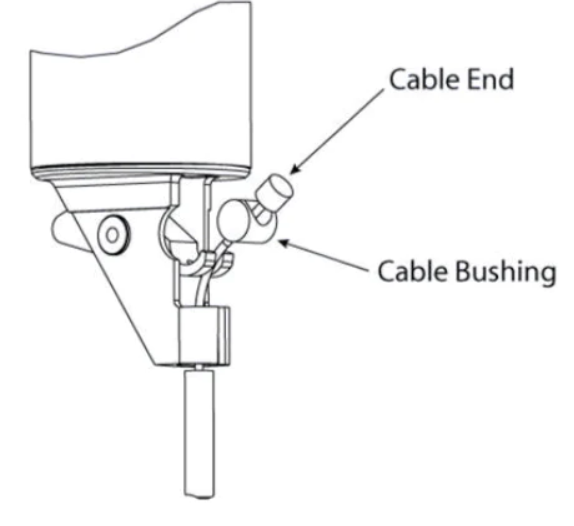
\includegraphics[width=1.0\textwidth]{bushing.png}
        \end{column}
    \end{columns}
\end{frame}


\section{Lab}
\frame{
    \frametitle{Lab This Week}

    \begin{enumerate}
        \item Create flange specified in the mechanical drawing
        \begin{enumerate}
            \item Add a 5 mm hex head set screw (other specifics, e.g., thread pitch, are arbitrary) to
            the flange collar to hold a rod in place
            \item Generate an assembly with a mocked rod part
            \item Generate a mechanical drawing based on your part
        \end{enumerate}
        \item Create the part and mechanical drawing for the Fox bushing
    \end{enumerate}

    Please submit everything through Gradescope.

}

\end{document}
